\documentclass[english]{tktltiki}
\usepackage[pdftex]{graphicx}
\usepackage{subfigure}
\usepackage{url}
\begin{document}
%\doublespacing
%\singlespacing
\onehalfspacing

\title{Car Automation, the future of self driving cars and ethical questions 
related to autonomous vehicles}
\author{Niki Ahlskog}
\date{\today}

\maketitle

\numberofpagesinformation{\numberofpages\ pages + \numberofappendixpages\ 
appendices}


\keywords{car, car automation, self awareness, self driving car, robot}

\begin{abstract}

Many manufacturers have all ready presented their solutions for self driving 
cars (also known as self-driving cars, autonomous vehicles or robot cars), but 
not a single one has been officially sold or accepted to be used in public 
roads. This report will have a look on the current situation of car automation. 
Can we expect to have self driving cars in public roads during the next 5 years 
or will it be more. What kind of difficulties are related to autonomous 
vehicles, for example how to program a logic in case of accident.


Most often there are no news about self driving cars, unless they crash. This 
leaves some ethical questions how cars should be programmed in case of 
collision. There are also different kind of autonomous vehicles coming in the 
future, for example heavy transport vehicles. What kind of problems this will 
create for autonomous vehicle creators? Global standards needs to be set for 
autonomous vehicles before letting them in traffic.

Many companies are currently putting a lot of effort to get autonomous vehicles 
on the road. Google, the technology company everyone knows is willing to put 
time and money for sensor technology, computer vision and GPS assistance. Uber, 
the cheaper taxi on demand would have huge benefits if they didn't need drivers. 
Uber is not creating the cars, but financing the technology. And for third, the 
Tesla electric cars. Tesla is trying to create a self driving car for consumers. 
The technology is among us, but how long it will take for public markets to see 
self driving autonomous vehicles?

This article will have a look on the motivations behind vehicle automation, how 
we could benefit about it, current situation, ethical questions, the downsides 
and the future of vehicle automation.


\end{abstract}

\mytableofcontents

\section{Introduction}
The already crowded race to put autonomous vehicles on the road may happen 
quicker than we thought. Mercedes-Benz's parent company just announced in April 
2017 that they are planning to release driver-free taxi service in as little as 
three years. Other companies are planning to also release self 
driving cars in the next five years. Google, Tesla and Uber have been working on 
the technology for many years. These companies will encounter a lot of 
challenges in order to put autonomous vehicles on the public roads. 

The benefits of autonomous vehicles are efficiency and safety. On the other hand it leaves 
people unemployed and leads to personal assistance questions. For example if 
elderly people need assistance in travel, there would be no driver to help. Or 
if the luggage is very heavy, or passenger is drunk there would be no one for 
them to help. 

There are also downsides, what happens in case of possible collision, who 
decides who lives and who dies? Will we have both, autonomous vehicles and 
ordinary cars driving on the some roads, or only fully automated vehicles to 
make things more simple for manufacturers? The autonomous vehicles are coming, 
that is for sure, but will it be in the next three years, or will it take even 
tens of years more? This article will answer most of the questions and have a 
look on the current situation and the future of car automation.

\section{Vehicle automation}
Autonomous vehicle, AVs, also known as self-driving car, or a robot car, is a 
vehicle which operates and drives solely on computer algorithm. There is no need 
for human interaction and the vehicle can operate from point A to B harmless. 

Autonomous vehicles can be compartmentalized in five levels \cite{transportpolicy}.


\begin{enumerate}
\item
First level of self 
driving vehicle is automating single functions. This includes devices such as 
cruise control, lane guidance and automated parallel parking. 
Still human driver is required to operate the vehicle and 
driver is fully responsible for all the actions.
\item
The second level is combined and automated functions \cite{transportpolicy}, for example function like 
adaptive cruise control with lane centering, which keeps the vehicle in the lane 
by following road marks and adapts the speed based on the car driving ahead. In 
the second level drivers are responsible for monitoring the roadway and are 
expected to start steering on demand. In level two driver can keep hands and 
foots of from the steering equipments but are required to operate the vehicle in 
varying conditions.
\item
Level three is a limited self driving \cite{transportpolicy}. It requires the driver to take controls 
under certain conditions, but most of the time the vehicle can operate itself. 
\item
Level four, self driving vehicle under specific conditions. In this level 
vehicle can operate under specified conditions \cite{transportpolicy}, for example drive from point A 
to point B
\item
Level five is the last level of autonomous vehicle. In this last level vehicle 
can operate on all conditions, no matter of weather, speed or road type. 
\cite{transportpolicy} Also it is possible that in the final level vehicles 
could have some sort of self awareness, for example finding best parking place 
nearby or pick up different persons in the meanwhile. This way people could use 
autonomous vehicles on demand.
\end{enumerate}

Most likely self operating vehicles gained much more attention in year 2010 when 
Google announced its automated driving program. \cite{heavyvehicle} However vehicle automation 
research has been active around the world since the concept of road vehicle 
automation was first introduced at the 1939 New York World's Fair's Norman Bel 
Geddes Futurama exhibit.

Self operating vehicles could be cars, road condition workers, like automatic 
snowblowers, heavy transportation vehicles or passenger coaches. This leads to 
different kind of use cases. For individual passenger cars the motivation to 
automate driving is to free the driver from tedious task, \cite{heavyvehicle} which would be 
considered as distraction otherwise. For heavy transportation the motivation 
could be saving on fuel and personnel costs, minimizing crashes and promising 
increased productivity.

In common all self operating vehicles share motivation for safety. \cite{heavyvehicle} Many car 
crashes are due to driver mistakes or equipment failure and maintenance issues. 
Self driving vehicle creators must understand different kind of crash scenarios 
and pay attention especially on level 2 functions. Simply by automating parts of 
the car functions may have much larger impact on safety.

The main idea of self driving vehicles seems to be clear. Less accidents, safety 
first, no driver mistakes, savings on fuel costs, improved traffic due to GPS 
navigation systems and real-time updates about traffic jams and accidents on the 
road.

Currently in (2017) many new vehicles have some sort of automated functions 
implemented. Even some older cars has functions like cruise control and parking 
sensors. Newer cars can park automatically and drive behind other cars, while 
electronics keep the distance automatically at defined point. Lane control is 
one of the newest features which steers the wheel automatically and keeps the 
car between lanes. Theoretically by following other car, driver is free from 
controls, however in practice it is not possible to drive from point A to point 
B without touching steering wheel.

Partially automated cars are all ready among us, but they are not as advanced as 
fully autonomous cars. Google has implemented level three vehicle, which have 
driven hundreds of kilometers without need for driver to touch controls. However 
majority of Googles self driving car testing has happened under strict 
conditions. Pre planned routes and there has always been driver available in 
case of system failure. \cite{transportpolicy} "Many manufacturers aspire to 
sell level four vehicles within few years" \cite{transportpolicy} but it would 
require strict requirements from governments and probably global rules on 
driving habits and traffic signs.   


\section{Autonomous vehicle technology}

In the future it is very likely that the vehicles doesn't only drive 
automatically, but also communicate with each other. \cite{trafficmodels} 
Communication between vehicles will be changing information, for example road 
conditions, weather and also fetching data from centralized servers. From 
centralized servers bots could distribute useful information to vehicles. 
Imagine your car finding the nearest free parking spot while you are doing your 
shoppings at shopping mall. 

\begin{figure}[h]
\ \newline
\begin{center}
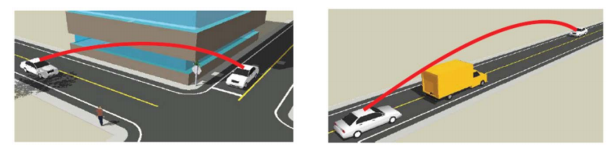
\includegraphics[width=0.9\textwidth]{nonlineofsight.png}
\caption{Non line of sight technology is about sharing information between vehicles in close. 
\cite{connectedvehicle}}
\label{non line of sight}
\end{center}
\end{figure}

In addition to changing information between vehicles and retrieving centralized 
data, \cite{trafficmodels} autonomous vehicles can contain hundreds of sensors. These sensors 
retrieve constantly information about the environment itself. Sensors plan what 
should be executed in the next step. Changing information between vehicles helps 
for example planning the computer what to do. For example sitting in traffic 
lights the car in front could inform your car that it is going to turn left, 
which helps planning what step should be  taken next. 

\begin{figure}[h]
\ \newline
\begin{center}
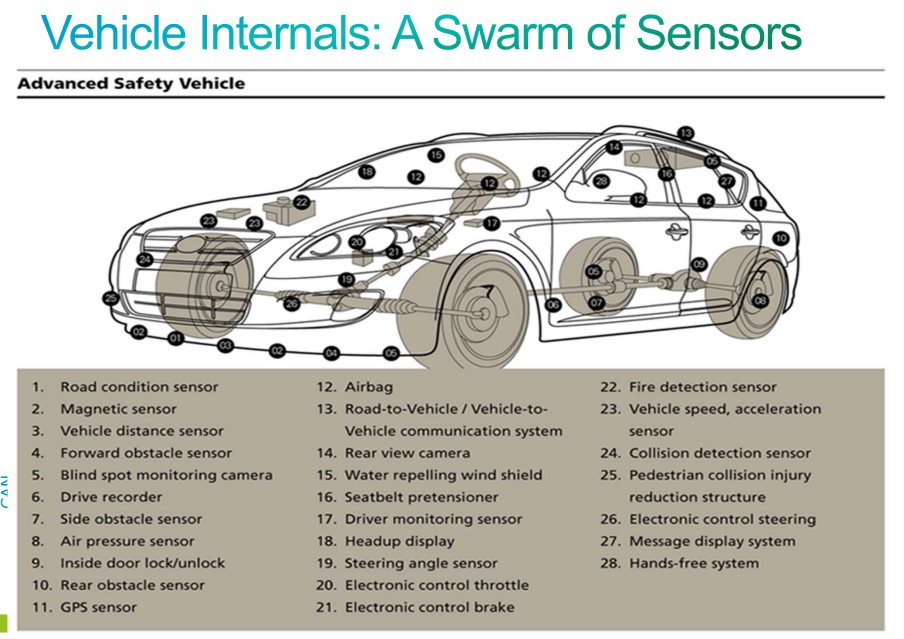
\includegraphics[width=0.9\textwidth]{vehicleinternals.png}
\caption{Vehicle internal sensors. 
\cite{connectedvehicle}}
\label{sensors}
\end{center}
\end{figure}

Autonomous vehicle sensors consist of for example laser range finder, which creates 3D-images 
of objects that helps the car see hazards along the way. Laser range finder also calculates 
how far an object is from the moving vehicle the same as sonar sensors work, how long it takes 
for the laser beam to return from the object it bounced from. Laser can also travel long distances, 
so it is possible to calculate distance from impressive 200 meters away.

Front and rear cameras help vehicle to see obstacles right in front or back of the vehicle. Cameras help on parking the vehicle, see pedestrians and other motorists close by. Geo-location sensor tracks vehicle position and works in harmony with the navigation and route system. 

Tires can have ultrasonic sensors as well. Ultrasonic sensors are implemented even in some of the current cars in the markets. Ultrasonic sensors in the tires helps the car to park automatically. Ultrasonic sensors will alert in case of collision. Inside the autonomous vehicle there will be a gyroscope which determines the car position. 

\begin{figure}[h]
\ \newline
\begin{center}
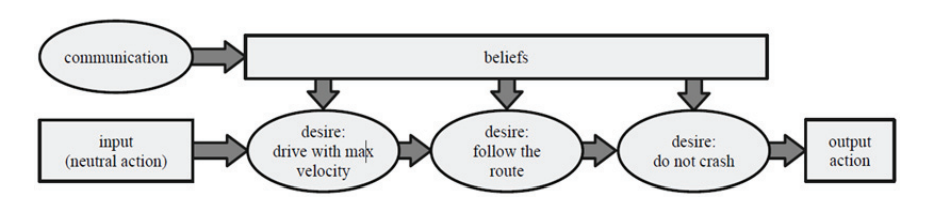
\includegraphics[width=0.9\textwidth]{process.png}
\caption{Deliberation process: how an action is designed. 
\cite{trafficmodels}}
\label{vehicle automation flow}
\end{center}
\end{figure}

In order for vehicle to drive autonomously it requires a lot of data, from sensors and servers. The deliberation process could be following as in the picture. Vehicle gets information from centralized servers, then makes assumptions on conditions and also takes into consideration the user interaction and desires. From the data collection vehicle calculates an optimal route, speed and velocity. As soon as the vehicle finishes processing of each individual step it executes them one by one.  

Autonomous vehicles will be programmed to understand traffic signs and in the future real life road behavior as well. For the data sharing centralized data-centers must be built. Autonomous vehicle sensors (embedded systems and sensors) will share information between other vehicles. Vehicle first need to process the data and decide which is useful information. For example bad road condition could be useful information. This information is then sent with mobile data as 3G, 4G, WiFi or some other similar technology to a distributed server. From distributed server the data will be stored in a data center or cloud server. From the cloud servers this information is passed to other vehicles after program logic decides what information should be shared and for which cars.  

As presented in the image below, infrastructure for autonomous vehicles could be the following, \cite{trafficmodels} Cars near by share information between, what actions they are going to take and notify others with some kind of Ad-Hoc technology. The overall conditions are shared with cellular data to centralized servers. From servers general information about weather and road conditions are sent back to the vehicles. 

\begin{figure}[h]
\ \newline
\begin{center}
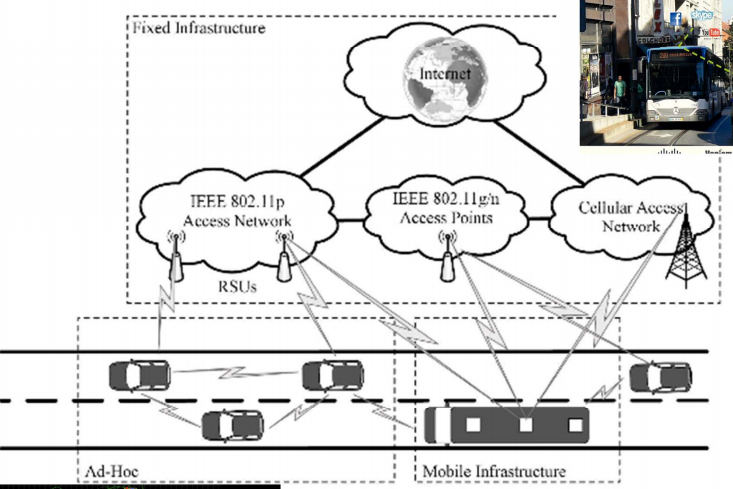
\includegraphics[width=0.9\textwidth]{infra.png}
\caption{Infrastructure for autonomous vehicles. 
\cite{trafficmodels}}
\label{infrastructure}
\end{center}
\end{figure}


\section{Vehicle sharing}
On the consumer or public side the future idea that automated car manufactures 
pursue is most likely reservation-based autonomous vehicles. It is widely known 
that for example Uber is putting huge amounts of money to the autonomous vehicle 
creation. Autonomous vehicles would allocate road capacity, reduce travelling 
costs and remove the need of own a personal vehicle. \cite{ondemand} "Automated 
mobility on demand is foreseen as the future of urban passenger mobility" 
\cite{ondemand} This would most likely require that all the cars in the traffic 
are either autonomous or then the cars should be so well made that they can 
adjust if there are conventional vehicles driving at the same time. Combined 
with mobility as a service it will open new possibilities on travelling and 
removes the need to own a vehicle. 

The impacts of shared travels are very 
difficult to predict. Autonomous vehicles could reduce vehicle ownership up to 
43 percent, and increase travel per vehicle up to 75 percent. 
\cite{transportpolicy} There are many reasons why vehicle users would still 
prefer a personal vehicle rather than shared, for example status, or if they 
frequently need to keep tools with them or transport some dirty stuff.


\section{Ethical questions and challenges}
One of the main challenges is the autonomous vehicle algorithms that decide what 
happens in case of collision. \cite{dilemma} Autonomous vehicles should reduce 
traffic accidents, but sometimes they have to choose between the evils. For 
example in the early steps there would be most likely both conventional cars and 
AV's in the traffic at the same time. In case of running over a pedestrian the 
car designer has to think about algorithm which decides if the car drives over 
the pedestrian or sacrifices itself and the passenger in order to save 
pedestrians. If the autonomous vehicle creators decide to create algorithm that 
saves the pedestrians by any means, this leads to a question if anyone would 
like to buy a vehicle that sacrifices the passenger for the greater good. Making 
these moral decisions is a formidable challenge.

Although these scenarios are very unlikely to happen if the traffic consists of 
autonomous vehicles only, there is still the risk that something will happen, as 
humans has created the vehicles and humans tend to make errors. Moreover if 
these scenarios will ever happen the algorithm must include decision rules about 
what to do in such cases. \cite{dilemma} Like in any software project, the 
computer program has to understand every possible case to be precise, efficient 
and not to end up with error because wrong user interaction. These types of 
"rules" need to be made well before selling autonomous vehicles in the global 
markets. It is also possible that governments need set some kind of standards 
for autonomous vehicles that everyone follows, like road signs and general 
driving  rules are very well thought to prevent accidents. This leads to a 
discussion to align moral algorithms with human values, like what kind of moral 
algorithm we are willing to accept as citizens and to be subjected to car 
owners. 

The social dilemma of autonomous vehicles article presents and interesting 
survey about autonomous vehicle algorithms. In the article they did a survey, 
and 76 percent of participants thought that it would be more moral for a vehicle 
to sacrifice passengers instead than kill ten pedestrians. \cite{dilemma} Also 
the approval of passenger sacrifice reduced when there were less pedestrians to 
save. The moral approval increased with the number of lives that could be saved. 
In addition to the morality of sacrifice it decreased if for example a family 
member was travelling with the vehicle.

Interesting fact about the survey is that even though most of the people voted 
autonomous vehicles should sacrifice the passenger for greater good they would 
still prefer a self protective vehicle if they personally owned it. 
\cite{dilemma} This is the social dilemma for autonomous vehicles and most 
likely the solution is going to be the best global outcome. Three groups in 
together may be able to solve the ethical dilemmas: \cite{differences} consumers who will buy 
autonomous vehicles, manufacturers that program the vehicles and also 
governments that may regulate programming algorithms. "Figuring out how to build 
ethical autonomous machines is one of the thorniest challenges in artificial 
intelligence today"

Even though autonomous vehicles sound very promising and everyone talks about 
reducing costs, there are also costs in autonomous vehicles that may have not 
been thought. If there are for example users in lower-density suburban areas are 
the costs same there when the vehicle drives back empty? Shared vehicles require 
frequent cleaning when passengers litter, spill some food and drinks or even 
smoke inside the vehicle. Vehicle seats will wear out, tires will wear out, 
vehicles may be vandalized and so forth. Lets assume one vehicle does 25-50 
trips per day. 5-15 percent of passengers leave some mess behind and cleaning it 
will cost 10 euros. This would lead to roughly 400 Euros per month as cleaning 
costs. Also services would reduce, there is no driver to help elder people or 
with heavy luggage. Autonomous vehicle doesn't ensure safe trip to the 
destination for example if traveller is drunk. Probably autonomous vehicles 
would have reduced comfort and privacy as well. In order to keep cars clean the 
seats and other comforts are minimized as in every public transport vehicle at 
the moment. No carpeted floors, fewer accessories and so on. Vehicles probably 
require some kind of security system, for example recording cameras which leads 
to reduced privacy. Cameras can prevent vandalism, but passengers will need to 
accept that all their actions are recorded during the travel. 


\section{Conclusion}
Despite the current level of autonomous vehicles a significant technical 
improvement is needed in order to achieve a fully autonomous vehicles driving in 
the public roads. \cite{transportpolicy} Failure in sensor or in computer 
program could be deadly for the passengers as well as other road users. Software 
in autonomous vehicle needs to be very robust and sensors require high 
performance. Several more years are required that the technology and software is 
advanced enough. Also the potential users need to gain confidence that fully 
autonomous vehicles an operate as expected under all conditions, for example in 
snow or foggy conditions. 

Autonomous Vehicle Implementation Predictions Implications for Transport 
Planning report presents a table, which shows the year, sales amount and use of 
autonomous vehicles. \cite{transportpolicy} In the article it is presented that 
by 2020 there would be a autonomous vehicle which is very expensive, and sales 
is only 2-5 percent of all cars. Just in ten years the price drops to moderate 
and the sales is from 20 to 40 percent. By 2050 autonomous vehicle is a standard 
and sales is up to 100 percent.

Autonomous vehicles will most likely arrive at some day, but it will still take 
many years. Deciding standards for the industry and to be sure about the safety 
of autonomous vehicles requires a lot of testing and effort. There has been no 
discussion with governments about regulations and not a single fully 
autonomously driving vehicles have been sold to public. The next ten years will 
give answers about autonomous vehicles and for sure, will be very exciting. As 
found in many articles, the downsides and challenges have been thought between 
manufacturers and most likely they are going to end up with the best possible 
algorithms and solutions in order to push autonomous vehicles on the public 
roads. 

If we look at the recent years, automation has only done good for humanity. It 
frees us from work we don't want to do. For some people driving is freedom, but 
in crowded cities the advantages of autonomous vehicles are just too good. For 
example the company Uber is very highly valuated in stock market and if they can 
get rid of the drivers who demand salary and cut the company revenue the company 
value will be blown. No wonder many other companies develop technology for 
autonomous vehicles. \cite{transportpolicy}  Autonomous vehicles will ease 
traffic, allow using transport more easily and effectively and maybe even get 
rid of the polluting fuels as the cars will most likely run with electricity. 
Autonomous vehicles can remove the need to own a personal vehicle, but still 
leads to some questions we do not have an answer at the moment. Only time will 
tell.


\nocite{*}
\bibliographystyle{tktl}
\bibliography{lahteet}

\lastpage

\appendices

\pagestyle{empty}

\end{document}



